\chapter{Model}
	\label{Chap:Model}
	\section{EIRENE}
		EIRENE is a Monte Carlo code used for simulating fusion plasma particles. Its first version was written in the scope of the PhD thesis by D. Reiter. It has been used on a variety of studies\footnote{For Example a B2-EIRENE and SOLPS numerical study of Iter divertors \cite{EirStudy} } in the fusion community. The following section contains a brief introduction to the capabilities of EIRENE, followed by the specific example case it was used to study in this work.\\
		~\\
		EIRENE simulates transport and plasma interaction of neutral particles in a fusion device given a plasma background. It is often used in connection with the EMC3\todo{Add citation} or SOLPS\footnote{SOLPS stands for Scrape-Off Layer Plasma Simulation, see \cite{SOLPS} for detailed information.} codes to study simulations of fusion plasma.\\
		~\\
		The Wang Chang-Uhlenbeck (WCU) equation \cite{WCU}, a multi species set of "Boltzmann"-type equations,\todo{this is also a direct quote from EIRENE manual, reword or quote??} is solved by EIRENE as described in \cite{EIRENE} chapter 1. This allows to calculate trajectories and mean free path length that can be used to simulate interactions in a standard Monte Carlo procedure\todo{More explanation necessary?}. The interactions of neutral particles can form source terms for plasma codes. To this end the Monte Carlo codes uses probabilities by considering effective cross sections and plasma chemistry reaction rates.\\
		Furthermore EIRENE is capable of calculating radiation transport and simulating charged particle movement.\footnote{Though since it is often used in conjunction with plasma codes this feature is less prominently known and hence used.} All of these features are available in arbitrary 3-dimensional geometries.\footnote{Please refer to the geometry section of the EIRENE manual \cite{EIRENE} for further information.}\\
		~\\
		In this work EIRENE is used in a one dimensional geometry with two surfaces. One perfectly reflective, simulating the outer wall, and one perfectly absorbing, simulating the core plasma. When particles are reflected they can cause atoms of the wall to be released as ions, which are redirected onto the wall by the surrounding magnetic field. The rate at which this happens is called a sputter rate.\\
		The geometry is chosen to be as simple as possible to minimize run time and thus allow for a production of big data sets. Furthermore the amount of input parameters has been reduced by assuming that ions and electrons have the same temperature $T_I =T_e$. This is a reasonable assumption depicting the source plasma in a thermal equilibrium.\\		
		The work of Mitja Beckers \cite{Beckers} used the very same model to investigate the erosion of the first wall. A more in depth introduction into the plasma physics background can be found in chapter 3 of his work and is not repeated here. Most of the concepts are rather elaborate and not suited to be summarized in a short manner. The following section will only highlight necessary parameter origins to give an insight as to the physical context of this work.
		
	\section{Plasma Profiles}
		For the inputs of EIRENE plasma profiles are needed, that can be dynamically provided by other algorithms like SOLPS or EMC3. Central piece of this work is to investigate if a substitute function can be found for the full range of possible plasma profiles by using big data methods. One can ascertain the physical limits of the parameters constituting the plasma profiles from tables \ref{Tab:ParameterT} and \ref{Tab:Parametern}. These limits are based on different phenomenons in plasma physics, explained by Mitja Beckers in his PhD thesis \cite{Beckers} and an example limitation is visualized in one of his graphics, which is depicted in \ref{Fig:Beckers_Constr} \todo{Look into source 55 from Becker PhD for english picture and source}.\\
		
		\begin{figure}
			\centering
			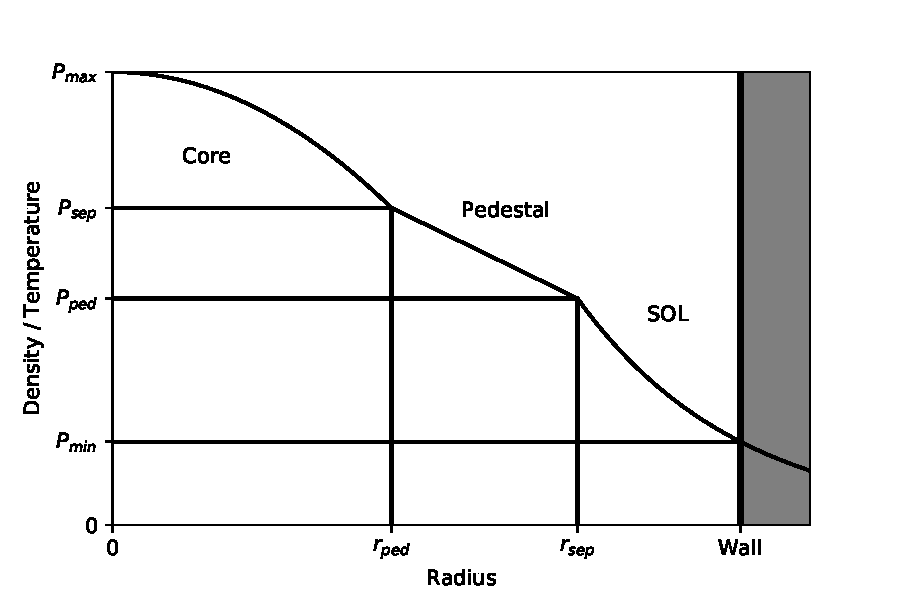
\includegraphics[width=0.8\textwidth]{./images/DensityPlot.pdf}
			\caption{Illustration of functional dependencies of temperature and density profiles according to equations \ref{EQ:TProf} and \ref{EQ:NProf}. Note that this schematic is not proportioned realistically, but has elongated pedestal and SOL regions for better visibility. Realistic values for the parameters can be found in tables \ref{Tab:ParameterT} and \ref{Tab:Parametern}.}
			\label{Fig:PlasmaProfile}
		\end{figure}
		
		\begin{figure}[ht]
			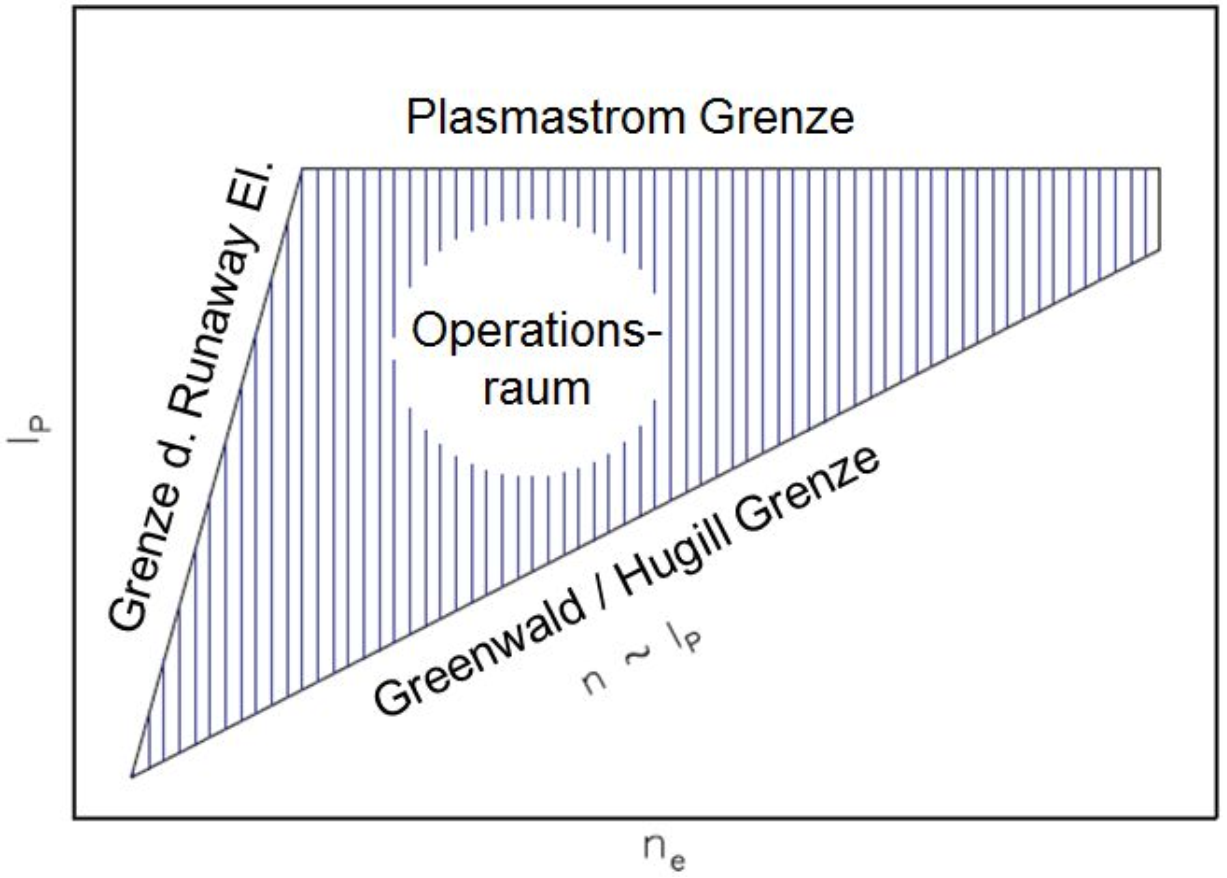
\includegraphics[width=.8\textwidth]{./images/Mitja_PlasmastromGrenze.png}
			\caption{Density and current limits for toroidal plasma devices, i.e. Tokamak reactors. The shaded area is the parameter space in which a plasma can be stably operated. Image taken from \cite{Beckers}}
			\label{Fig:Beckers_Constr}
		\end{figure} 
	    
	                     
		\FloatBarrier
		
 		Table \ref{Tab:ParameterT} shows the breakdown of temperture profile parameters used in equation \ref{EQ:TProf}, ordered according to the input into the EIRENE code.
		
		\begin{equation}
			T(r) =
			\begin{cases}
				T_{\textrm{ped}} + (T_0 - T_{\textrm{ped}}) \left(1 - \left(\frac{r}{r_{\textrm{ped}}} \right)^2 
				\right)^{\alpha_T} &\textrm{if $r \le r_{\textrm{ped}}$}\\
				mr + b & \textrm{if $r_{\textrm{ped}} < r \le a$}\\
				\textrm{max}\left(T_{\textrm{sed}} \cdot e^{\left( \frac{-(r-a)}{\lambda_{T_1}} \right)} , 
				T_{min} \right) & \textrm{if $r > a$ and $T > T_{\textrm{min}}$}\\
				T_{\textrm{min}} \cdot e^{\left( \frac{-(r-a)}{\lambda_{T_2}} \right)} & \textrm{other cases} \\
			\end{cases}
			\label{EQ:TProf}
		\end{equation}
		~\\
		with \\
		\begin{equation*}
			m = \frac{T_{\textrm{sed}} - T_{\textrm{ped}}}{\Delta_{\textrm{ped}}}, \quad b = T_{\textrm{sed}} - ma
		\end{equation*}
		
		\begin{figure}
			\caption{Temperature Profile Parameter Overview}
			\begin{tabular}[width=.8\textwidth]{c|c|c|c|l}
				Name & Unit & Min & Max & Note \\
				\hline
				T$_0$ & eV & $2 \cdot 10^4$ &  $3 \cdot 10^4$ & Core value \\
				$\rho_{ped}$ & 1 & $0.9$ &  $0.96$ & Relative Distance to Pedestal region \\
				$\alpha_{T}$ & q & $0.5$ &  $2$ & Core profile Shape Parameter \\
				$R_{sep}$ & cm & $264.3$ &  $264.3$ & Small Radius \\
				T$_{ped}$ & eV & $0.3 \cdot 10^4$ &  $0.8 \cdot 10^4$ & Upper Pedestal Value \\
				T$_{sep}$ & eV & $0.1 \cdot 10^4$ &  $0.5 \cdot 10^4$ & Lower Pedestal Value = Upper Seperatrix Value \\
%				P7 & NA & NA &  NA & Zur Zeit nicht in Benutzung \\
%				P8 & NA & NA &  NA & Zur Zeit nicht in Benutzung \\
%				P9 & NA & NA &  NA & Zur Zeit nicht in Benutzung \\
				$\lambda_T$ & cm & $0.1$ &  $1.0$ & Penetration depth at $\rho \ge 1$\\
				T$_{min}$ & eV & $5$ &  $20$ & Ceiling in SOL\\
				$\lambda_{T_2}$ & cm & $ $ & $ $ & Penetration depth At low temperatures in SOL\\
%				P12 & 1 & $ $ & $ $ & scaling factor
			\end{tabular}
			\label{Tab:ParameterT}
		\end{figure}
		
		\subsection{Density Profile}
		Analogue to the parameters of temperature profile table \ref{Tab:Parametern} shows the breakdown of parameters used in equation \ref{EQ:NProf} in order of the EIRENE input file.
		
		\begin{equation}
			n(r) =
			\begin{cases}
				n_{\textrm{ped}} + (n_0 - n_{\textrm{ped}}) \left(1 - \left(\frac{r}{r_{\textrm{ped}}}\right)^2 
				\right)^{\alpha_n} & \textrm{if $r \le r_{\textrm{ped}}$}\\
				mr + b & \textrm{if $r_{\textrm{ped}} < r \le a$} \\
				n_{\textrm{sed}} \cdot e^{\left(\frac{-(r-a)}{\lambda_n}\right)} & \textrm{other cases}
			\end{cases}
			\label{EQ:NProf}
		\end{equation}
		~\\
		with\\
		\begin{equation*}
			m = \frac{n_{\textrm{sed}} - n_{\textrm{ped}}}{\Delta_{\textrm{ped}}}, \quad b = n_{\textrm{sed}} - ma
		\end{equation*}
		
		\begin{figure}
			\caption{Overview of density profile parameters}
			\begin{tabular}[width=\textwidth]{c|c|c|c|l}
				Name & Unit & Min & Max & Note \\
				\hline
				n$_0$ & $10^{14}$/cm$^3$ & $1$ &  $1.4$ & central value \\
				$\rho_{ped}$ & 1 & $0.9$ &  $0.96$ & Relative Distance to pedestal region \\
				$\alpha_{n}$ & 1 & $0.3$ &  $0.7$ & Core Profile Shape Parameter \\
				$R_{sep}$ & cm & $264.3$ &  $264.3$ & Small Radius \\
				n$_{ped}$ & $10^{14}$/cm$^3$ & $0.56$n$_0$ &  $0.78$n$_0$ & Upper Pedestal value \\
				n$_{sep}$ & $10^{14}$/cm$^3$ & $0.17$n$_{ped}$ &  $0.24$n$_{ped}$ & Lower Pedestal value = Upper Seperatrix value \\
%				P7 & NA & NA &  NA & Zur Zeit nicht in Benutzung \\
%				P8 & NA & NA &  NA & Zur Zeit nicht in Benutzung \\
%				P9 & NA & NA &  NA & Zur Zeit nicht in Benutzung \\
				$\lambda_n$ & cm & $1.0$ &  $20.0$ & Penetration depth at $\rho \ge 1$\\
%				n$_{min}$ & $10^{14}$/cm$^3$ & $0$ &  $0$ & Ceiling in SOL\\
%				P12 & 1 & $ $ & $ $ & Scaling factor
			\end{tabular}
			\label{Tab:Parametern}
		\end{figure}
		
		The input parameters for EIRENE that define the background plasma and geometry will be used as inputs and the sputter rate will be used as the label of the data sets used in this work. The following section talks about how to make intelligent choices on sampling from the parameter space to improve coverage of high dimensional spaces with sparse data. This might not seem necessary for the relatively basic model of this work, but is a conceptual improvement for further projects with more complicated geometries and additional parameters.
		
	\section{Choice of sampling set}
		Since the parameter space is high dimensional, the training points have not been selected randomly. Randomly sampled points might form clusters, which could skew the training towards a subsection of the parameter space. To avoid this a low discrepancy sequence, namely the Sobol sequence, is used to sample training data.\footnote{For a more detailed explanation of the Sobol sequence and its use cases please refer to \cite{ModernCompFinance} chapter 5, section 4: 'Better Random Numbers'.} It is a sequence in base 2 that form successively finer uniform partitions of the given space. Due to this attribute observations on the influence of the size of training data set is formed on base 2 bench marks instead of intuitive base ten orders of magnitude.\\
		The following figure \ref{Fig:512Dist} illustrates the clustering of randomly drawn data points in comparison to the Sobol sequence:
		\begin{figure}
			\centering
			\begin{subfigure}{.48\textwidth}
				\centering
				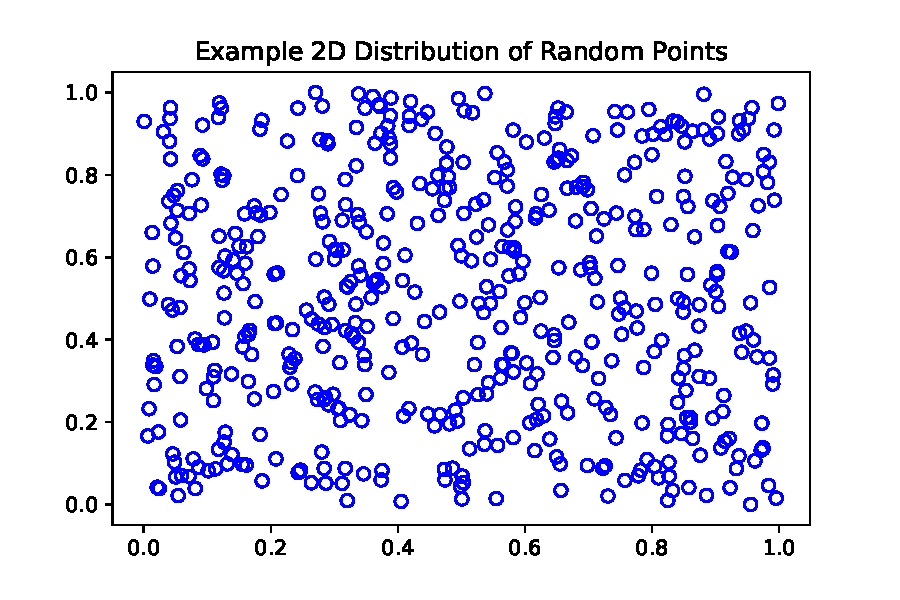
\includegraphics[width=\textwidth]{images/2D_Dist_Rand512.pdf}
				\subcaption{512 2D randomly generated data points.}
				\label{Fig:DistRand}
			\end{subfigure}
			\begin{subfigure}{.48\textwidth}
				\centering
				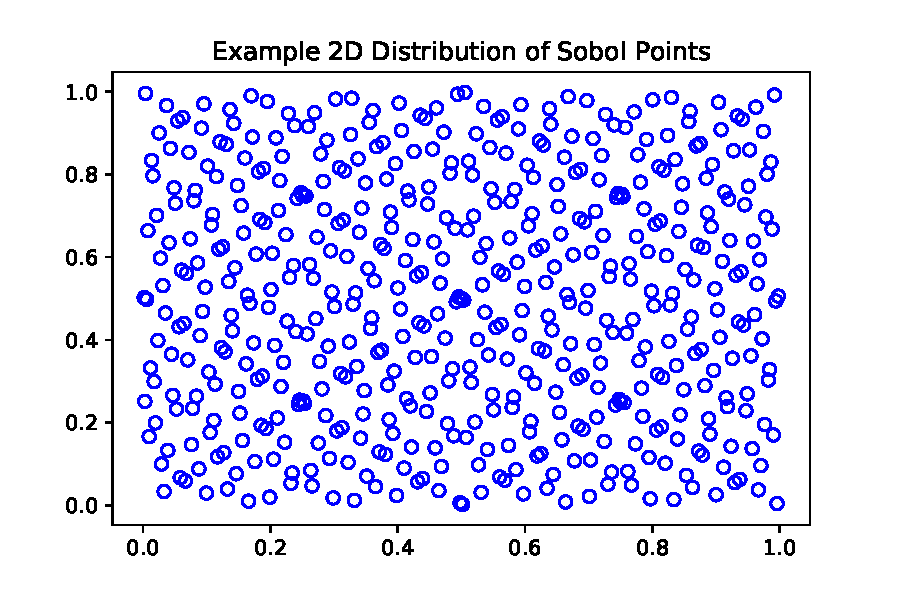
\includegraphics[width=\textwidth]{images/2D_Dist_Sobol512.pdf}
				\subcaption{First 512 Sobol points.}
				\label{Fig:DistSobol}
			\end{subfigure}
			\caption{Comparison of data point distribution to illustrate clustering of randomly drawn samples.}
			\label{Fig:512Dist}
		\end{figure}
		Especially in high dimensional spaces where data is often sparse it is important to make sure that the data is sufficiently spaced in order to adequately represent the parameter space.\\
		~\\
		The validation and test data were sampled from a random distribution\footnote{Using pseudo random generator from numpy standart library, based on Mersenne-Twister generator.} to ensure systematics from the training data do not influence network performance evaluation.
		